\documentclass[tikz,border=1.14mm]{standalone}
\usepackage{pgfplots}
\pgfplotsset{compat=1.15}
\begin{document}

	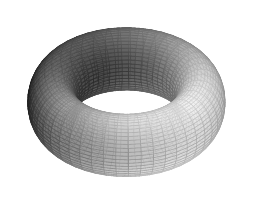
\begin{tikzpicture}[scale=0.5]
		\begin{axis}[colormap/blackwhite,
			view={30}{60},axis lines=none
			]
			% Plot the surface
			\addplot3[surf,opacity=0.7,
			samples=50, point meta=x+3*z*z-0.25*y,
			domain=0:2*pi,y domain=0:2*pi,
			z buffer=sort]
			({(3+cos(deg(x)))*cos(deg(y))}, 
			{(3+cos(deg(x)))*sin(deg(y))}, 
			{sin(deg(x))});
			
		\end{axis}
		
	\end{tikzpicture}
	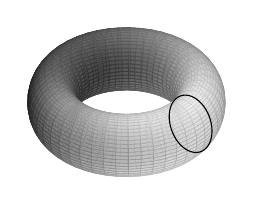
\begin{tikzpicture}[scale=0.5]
		\begin{axis}[colormap/blackwhite,
			view={30}{60},axis lines=none
			]
			% Plot the surface
			\addplot3[surf,opacity=0.7,
			samples=50, point meta=x+3*z*z-0.25*y,
			domain=0:2*pi,y domain=0:2*pi,
			z buffer=sort]
			({(3+cos(deg(x)))*cos(deg(y))}, 
			{(3+cos(deg(x)))*sin(deg(y))}, 
			{sin(deg(x))});
			
			% Plot the vertical line
			\addplot3[domain=0:2*pi, samples=50, x=0, black, thick]
			({(3+cos(deg(x)))*cos(deg(0))}, 
			{(3+cos(deg(x)))*sin(deg(0))}, 
			{sin(deg(x))});
		\end{axis}
		
	\end{tikzpicture}
	
	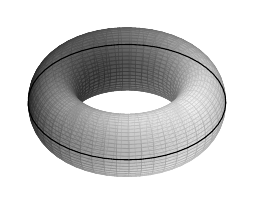
\begin{tikzpicture}[scale=0.5]
		\begin{axis}[colormap/blackwhite,
			view={30}{60},axis lines=none
			]
			% Plot the surface
			\addplot3[surf,opacity=0.7,
			samples=50, point meta=x+3*z*z-0.25*y,
			domain=0:2*pi,y domain=0:2*pi,
			z buffer=sort]
			({(3+cos(deg(x)))*cos(deg(y))}, 
			{(3+cos(deg(x)))*sin(deg(y))}, 
			{sin(deg(x))});
			
			% Plot the horizontal line
			\addplot3[domain=0:2*pi, samples=50, y=0, black, thick]
			({(3+cos(deg(0)))*cos(deg(x))}, 
			{(3+cos(deg(0)))*sin(deg(x))}, 
			{sin(deg(0))});
		\end{axis}
		
	\end{tikzpicture}
	
	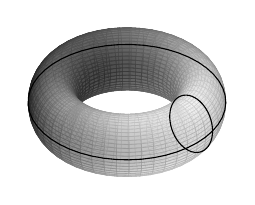
\begin{tikzpicture}[scale=0.5]
		\begin{axis}[colormap/blackwhite,
			view={30}{60},axis lines=none
			]
			% Plot the surface
			\addplot3[surf,opacity=0.7,
			samples=50, point meta=x+3*z*z-0.25*y,
			domain=0:2*pi,y domain=0:2*pi,
			z buffer=sort]
			({(3+cos(deg(x)))*cos(deg(y))}, 
			{(3+cos(deg(x)))*sin(deg(y))}, 
			{sin(deg(x))});
			
			% Plot the horizontal line
			\addplot3[domain=0:2*pi, samples=50, y=0, black, thick]
			({(3+cos(deg(0)))*cos(deg(x))}, 
			{(3+cos(deg(0)))*sin(deg(x))}, 
			{sin(deg(0))});
			
			% Plot the vertical line
			\addplot3[domain=0:2*pi, samples=50, x=0, black, thick]
			({(3+cos(deg(x)))*cos(deg(0))}, 
			{(3+cos(deg(x)))*sin(deg(0))}, 
			{sin(deg(x))});
		\end{axis}
		
	\end{tikzpicture}
\end{document}

%--------------------------

\begin{figure}
	
	\begin{center}
	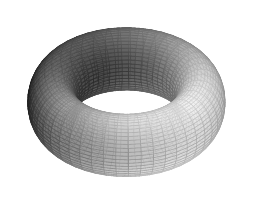
\begin{tikzpicture}[scale=0.5]
		\begin{axis}[colormap/blackwhite,
			view={30}{60},axis lines=none
			]
			% Plot the surface
			\addplot3[surf,opacity=0.7,
			samples=50, point meta=x+3*z*z-0.25*y,
			domain=0:2*pi,y domain=0:2*pi,
			z buffer=sort]
			({(3+cos(deg(x)))*cos(deg(y))}, 
			{(3+cos(deg(x)))*sin(deg(y))}, 
			{sin(deg(x))});
			
		\end{axis}
		
	\end{tikzpicture}
	\end{center}

\caption{--}
\label{fig:Torus}
\end{figure}

\begin{figure}
	
	\begin{center}
		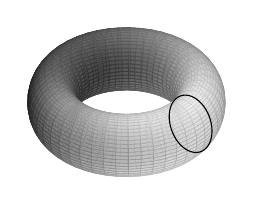
\begin{tikzpicture}[scale=0.5]
			\begin{axis}[colormap/blackwhite,
				view={30}{60},axis lines=none
				]
				% Plot the surface
				\addplot3[surf,opacity=0.7,
				samples=50, point meta=x+3*z*z-0.25*y,
				domain=0:2*pi,y domain=0:2*pi,
				z buffer=sort]
				({(3+cos(deg(x)))*cos(deg(y))}, 
				{(3+cos(deg(x)))*sin(deg(y))}, 
				{sin(deg(x))});
				
				% Plot the vertical line
				\addplot3[domain=0:2*pi, samples=50, x=0, black, thick]
				({(3+cos(deg(x)))*cos(deg(0))}, 
				{(3+cos(deg(x)))*sin(deg(0))}, 
				{sin(deg(x))});
			\end{axis}		
		\end{tikzpicture}
	\end{center}
	
	\caption{--}
	\label{fig:Torus1}
\end{figure}


\begin{figure}
	
	\begin{center}
		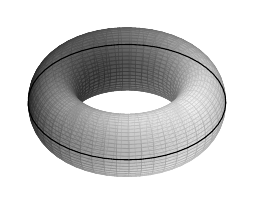
\begin{tikzpicture}[scale=0.5]
			\begin{axis}[colormap/blackwhite,
				view={30}{60},axis lines=none
				]
				% Plot the surface
				\addplot3[surf,opacity=0.7,
				samples=50, point meta=x+3*z*z-0.25*y,
				domain=0:2*pi,y domain=0:2*pi,
				z buffer=sort]
				({(3+cos(deg(x)))*cos(deg(y))}, 
				{(3+cos(deg(x)))*sin(deg(y))}, 
				{sin(deg(x))});
				
				% Plot the horizontal line
				\addplot3[domain=0:2*pi, samples=50, y=0, black, thick]
				({(3+cos(deg(0)))*cos(deg(x))}, 
				{(3+cos(deg(0)))*sin(deg(x))}, 
				{sin(deg(0))});
			\end{axis}
			
		\end{tikzpicture}
	\end{center}
	
	\caption{--}
	\label{fig:Torus2}
\end{figure}


\begin{figure}
	
	\begin{center}
		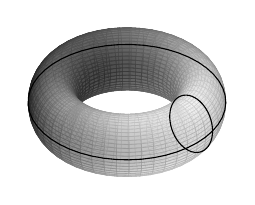
\begin{tikzpicture}[scale=0.5]
		\begin{axis}[colormap/blackwhite,
			view={30}{60},axis lines=none
			]
			% Plot the surface
			\addplot3[surf,opacity=0.7,
			samples=50, point meta=x+3*z*z-0.25*y,
			domain=0:2*pi,y domain=0:2*pi,
			z buffer=sort]
			({(3+cos(deg(x)))*cos(deg(y))}, 
			{(3+cos(deg(x)))*sin(deg(y))}, 
			{sin(deg(x))});
			
			% Plot the horizontal line
			\addplot3[domain=0:2*pi, samples=50, y=0, black, thick]
			({(3+cos(deg(0)))*cos(deg(x))}, 
			{(3+cos(deg(0)))*sin(deg(x))}, 
			{sin(deg(0))});
			
			% Plot the vertical line
			\addplot3[domain=0:2*pi, samples=50, x=0, black, thick]
			({(3+cos(deg(x)))*cos(deg(0))}, 
			{(3+cos(deg(x)))*sin(deg(0))}, 
			{sin(deg(x))});
		\end{axis}
		
		\end{tikzpicture}
	\end{center}
	
	\caption{--}
	\label{fig:Torus3}
\end{figure}

